\documentclass[a4paper,10pt]{article}

\usepackage[utf8]{inputenc} %
\usepackage[english]{babel}
\usepackage{fontenc}
\usepackage{graphicx}
\usepackage{amsfonts}
\usepackage{hyperref}
\usepackage{amssymb}
\usepackage{fullpage}
% \usepackage[ruled,vlined,linesnumbered]{algorithm2e}
\usepackage{float}
\usepackage{amsthm}
\usepackage{amsmath}
\usepackage{amssymb}
\usepackage{mathrsfs}
\usepackage{enumerate}
% \usepackage{wrapfig}
% \providecommand{\SetAlgoLined}{\SetLine}
% \providecommand{\DontPrintSemicolon}{\dontprintsemicolon}
\author{M1-MPRI Projet Génie Logiciel}
\date{Le 25/10/13}
\title{Délivrable I
}
% \theoremstyle{definition}
% \newtheorem{lemma}{Lemme}
% % \newtheorem{proposition}{Propriété}[chapter]
% % \newtheorem{definition}{Définition}[chapter]
% % \newtheorem{example}{Exemple}[chapter]
% % \newtheorem{cor}{Corollaire}[chapter]
% % \newtheorem{theorem}{Théorème}[chapter]
% \theoremstyle{definition}
\usepackage{tikz}
\usetikzlibrary{arrows}
\usepackage{fullpage}
\usepackage{empheq}
%  
% \newlength\dlf  % Define a new measure, dlf
% \newcommand\alignedbox[2]{
% % Argument #1 = before & if there were no box (lhs)
% % Argument #2 = after & if there were no box (rhs)
% &  % Alignment sign of the line
% {
% \settowidth\dlf{$\displaystyle #1$} 
%     % The width of \dlf is the width of the lhs, with a displaystyle font
% \addtolength\dlf{\fboxsep+\fboxrule} 
%     % Add to it the distance to the box, and the width of the line of the box
% \hspace{-\dlf} 
%     % Move everything dlf units to the left, so that & #1 #2 is aligned under #1 & #2
% \boxed{#1 #2}
%     % Put a box around lhs and rhs
% }
% }
% \theoremstyle{remark}
% % \newtheorem{req}{Remarque}[chapter]
% % \newtheorem{nota}{Notation}[chapter]

\tikzset{
    punkt/.style={
           rectangle,
           rounded corners,
           draw=black, very thick,
           text width=5em,
           minimum height=2em,
           text centered},
               punkt2/.style={
           rectangle,
           draw=pink, very thick,
           text width=5em,
           minimum height=2em,
           text centered},
  punktsi/.style={
           rectangle,
           rounded corners,
           draw=green, very thick,
           text width=5em,
           minimum height=2em,
           text centered},
             punktre/.style={
           rectangle,
           rounded corners,
           draw=blue, very thick,
           text width=5em,
           minimum height=2em,
           text centered},
             punktsc/.style={
           rectangle,
           rounded corners,
           draw=cyan, very thick,
           text width=5em,
           minimum height=2em,
           text centered},
             punktgr/.style={
           rectangle,
           rounded corners,
           draw=magenta, very thick,
           text width=5em,
           minimum height=2em,
           text centered},
           punktgrd/.style={
           rectangle,dashed,
           rounded corners,
           draw=magenta, very thick,
           minimum width = 2cm
           minimum height= 2cm,
           text centered},
             punktge/.style={
           rectangle,
           rounded corners,
           draw=yellow, very thick,
           text width=5em,
           minimum height=2em,
           text centered},
             punktmu/.style={
           rectangle,
           rounded corners,
           draw=red, very thick,
           text width=5em,
           minimum height=2em,
           text centered},
  treenode/.style = {align=center, inner sep=0pt, text centered,
    font=\sffamily},
  arn_n/.style = {treenode, circle , white, font=\sffamily\bfseries, draw=black,
    fill=black, text width=1.5em},% arbre rouge noir, noeud noir
  arn_r/.style = {treenode, circle , red, draw=red, 
    text width=1.5em, very thick},% arbre rouge noir, noeud rouge
  arn_x/.style = {treenode, rectangle, draw=black,
    minimum width=1em, minimum height=1em},% arbre rouge noir, nil
  arn_b/.style = {treenode, circle , blue, draw=blue, 
    text width=1.5em, very thick},
  arn_g/.style = {treenode, circle , green, draw=green, 
    text width=1.5em, very thick},
  arn_y/.style = {treenode, circle , yellow, draw=yellow, 
    text width=1.5em, very thick},
    arn_pu/.style = {treenode, circle , purple, draw=purple, 
    text width=1.5em, very thick},
    arn_pi/.style = {treenode, circle , pink, draw=pink, 
    text width=1.5em, very thick},
    arn_rb/.style = {treenode, circle , red, draw=red, 
    text width=2.5em, very thick}
    }% arbre rouge noir, noeud rouge}
    
\begin{document}
\maketitle
\tableofcontents

\section{Introduction}
\section{Architecture générale}
\subsection{Les différentes composantes et leurs interfaces}
% \begin{figure}[h]
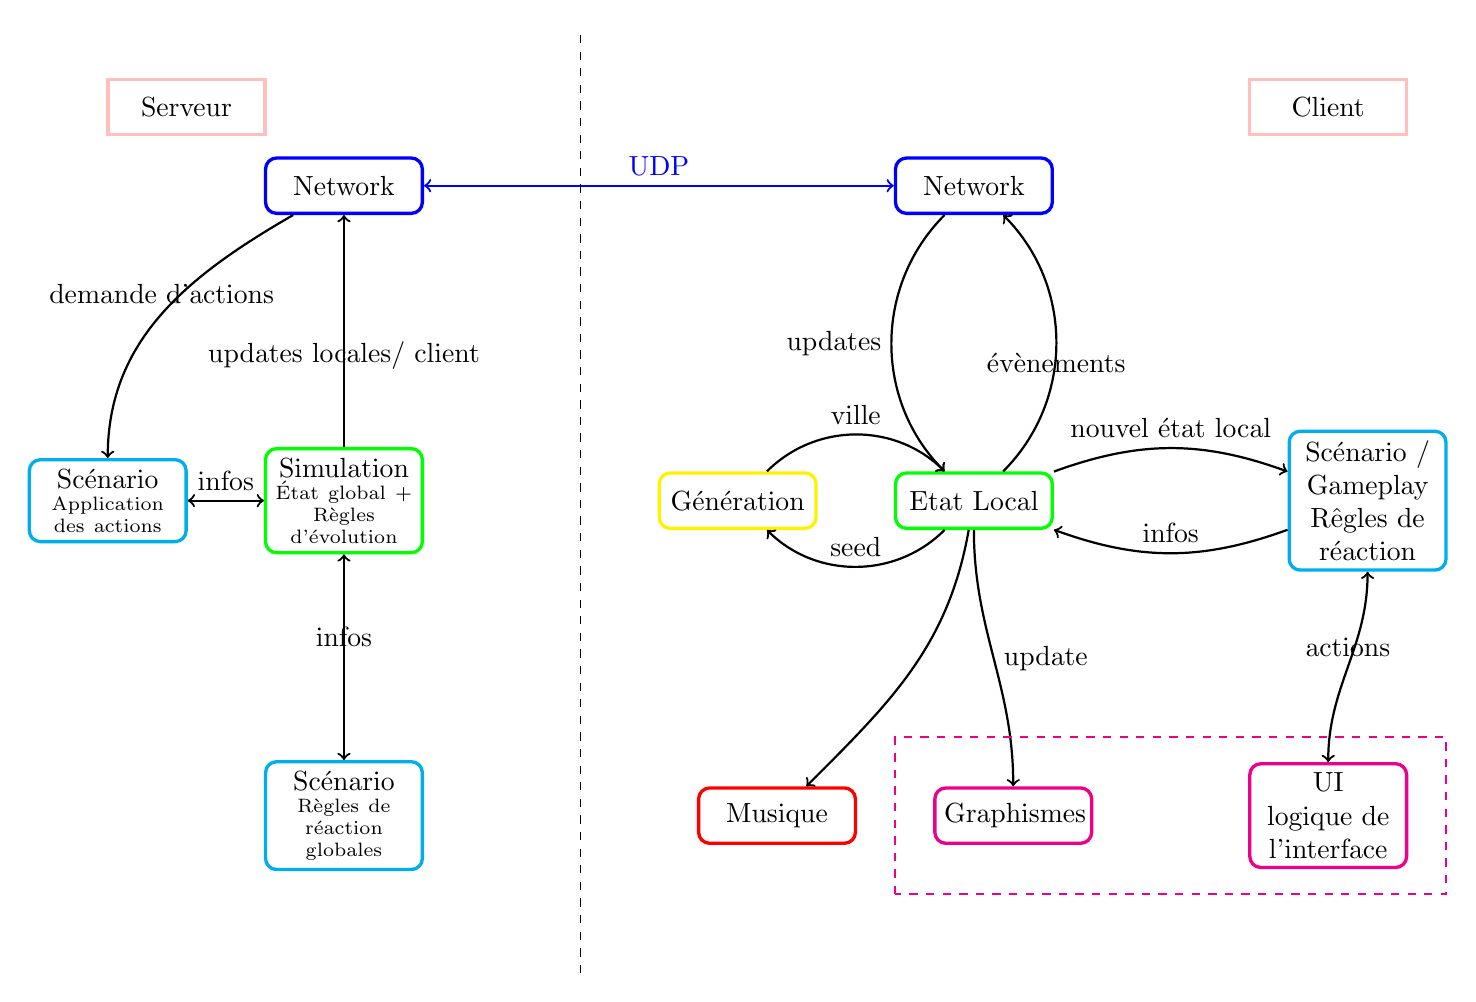
\begin{tikzpicture}
      \node[punktsi] (0) at (3,0) {Etat Local};
      \node[punktge] (1) at (0,0) {Génération};
      \node[punktmu] at (0.5,-4) (2) {Musique};
      \node[punktgr] at (3.5,-4) (3) {Graphismes};
      \node[punktgr] at (7.5,-4) (4) {UI \\ logique de l'interface};
      \node[punktsc] at (8,0) (5) {Scénario / Gameplay \\ Rêgles de réaction};
      \node[punktre] at (3,4) (6) {Network};
      \node[punktsi] at (-5,0) (7) {Simulation \\ {\scriptsize État global + \\ Règles d'évolution\\}};
      \node[punktsc] at (-5,-4) (8) {Scénario \\ {\scriptsize Règles de réaction globales\\}};
      \node[punktre] at (-5,4) (10) {Network};
      \node[punkt2] at (7.5,5) {Client};
      \node[punkt2] at (-7,5) {Serveur};
%       \node[punkt2] at (5.5,-4) {};
      \node[punktsc] at (-8,0) (11){Scénario \\ {\scriptsize Application des actions\\}};
      \draw[-,black,dashed] (-2,-6) -- (-2,6);
      \draw[->,black,thick] (1) to[out=45,in=135] node [midway,above] {ville} (0);
      \draw[->,black,thick] (0) to[out=225,in=-45] node [midway,above] {seed} (1);
      \draw[->,black,thick] (0) to[out=260,in=45] (2);
      \draw[->,black,thick] (0) to[out=270,in=90] node [midway,right] {update} (3);
%       \draw[->,black,thick] (0) to[out=-45,in=135] node [midway,left] {update} (4);
      \draw[->,black,thick] (0) to[out=20,in=160] node [midway,above] {nouvel état local} (5);
      \draw[->,black,thick] (5) to[out=200,in=-20] node [midway,above] {infos} (0);
      \draw[<->,black,thick] (4) to[out=90,in=-90] node [midway,above] {actions} (5);
%       \draw[->,black,thick] (4) to[out=180,in=0] node [midway,above] {update} (3);
      \draw[->,black,thick] (0) to[out=45,in=-45] node [midway,below] {évènements} (6);
      \draw[->,black,thick] (6) to[out=-135,in=135] node [midway,left] {updates} (0);
      \draw[<->,blue,thick] (6) to[out=180,in=0] node [midway,above] {UDP} (10);
%       \draw[->,black,thick] (10) to[out=-135,in=135] node [midway,above] {actions client} (7);
      \draw[->,black,thick] (7) to node [midway,below] {updates locales \\ / client} (10);
      \draw[<->,black,thick] (8) to[out=90,in=-90] node [midway,above] {infos} (7);
      \draw[<->,black,thick] (11) to[out=0,in=180] node [midway,above] {infos} (7);
      \draw[<-,black,thick] (11) to[out=90,in=-150] node [midway,above] {demande d'actions} (10);
      \draw[magenta,thick,dashed] (2,-5) rectangle (9,-3);
\end{tikzpicture}
% \caption{Structure \& interactions des composantes}
% \end{figure}

\begin{figure}[h]
\centering
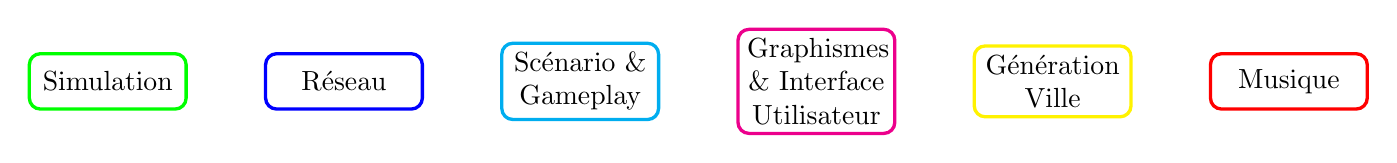
\begin{tikzpicture}
\node[punktsi] at (0,0) {Simulation};
\node[punktre] at (3,0) {Réseau};
\node[punktsc] at (6,0) {Scénario \& Gameplay};
\node[punktgr] at (9,0) {Graphismes \& Interface Utilisateur};
\node[punktge] at (12,0) {Génération Ville};
\node[punktmu] at (15,0) {Musique};
\end{tikzpicture}
 \caption{Code couleur des différents groupes de travail}
\end{figure}
\subsection{Choix technologiques}
\begin{itemize}
 \item Langage : \verb!C++!
 \item Bibliothèque Graphique : SFML
 \item Logiciel de versionnement : Git
 \item Hébergement : GitHub (\href{https://github.com/ProjetM1MPRI2013/central}{https://github.com/ProjetM1MPRI2013/central})
\end{itemize}
\subsection{Responsabilités globales}
\begin{itemize}
 \item Coordination : Adrien Husson
 \item Infrastructure : Matthieu Journault
 \item Support Technique : Adrien Koutsos
 \item Documentation utilisateur : Lucas Randazzo
\end{itemize}

\section{Description des sous projets}
\subsection{Simulation}
\subsection{Réseau}
\paragraph{Membres du sous-projet} Denys Kanunikov \verb!kanunikov-denys!. Marc Heinrich \verb!mheinric!.
\paragraph{}
On adopte une architecture type client/serveur. Ce sous-projet est responsable de la synchonisation des evenements et des données entre le serveur et les différents clients.

Sur le serveur, on effectue tous les calculs liés à la simulation (positions des personnages par ex). Les résultats de ces calculs sont ensuite envoyés de temps en temps à tous les clients, qui mettent à jour les données dont ils disponsent.

Coté serveur, il s'agit de mettre à disposition des méthodes pour la mise en place du serveur, la réception de commande des clients, et l'envoie de données pertinentes aux clients (on n'envoie pas l'état complet du monde au client, mais juste les données qui lui sont utiles, pour un joueur terroriste, la position des personnages autours de lui par exemple). Coté client, il faut recevoir ces données, et etre capable d'en tenir compte pour interpoler/extrpoler les donnees importantes (le taux de rafraichissement de l'écran sera beaucoup plus important que le taux de transfert par le réseau).

Il y a une interface importante avec la partie simulation, pour la façon dont sont représentées l'état du jeu, coté client et coté serveur, ainsi que sur le type d'evenements qui doivent etre transmis au seveur.

Interface : (provisoire, c'est juste pour donner une idée de ce qu'il faudra implémenter)
\begin{enumerate}
 \item Client : \begin{enumerate}
        \item \verb!createClient(ClientInfo)! cree un client à partir d'informations (nom, addresse du serveur pour se connecter ....) et essaye de le connecter au seveur.
        \item \verb!recieveUpdates()! regarde si il y a des données du serveur à recevoir, et si c'est le cas, les 'appliquer' pour qu'elles puissent etre prises en compte lors des affichages suivants.
        \item \verb!sendEvent(Evenement)! Envoie un evenement au serveur. Non blocant
       \end{enumerate}
\item Serveur : \begin{enumerate}
                 \item \verb!sendEvent(Evenement)! Envoie un evenement au serveur. Non blocant
                 \item \verb!sendState(Etat, joueur)! Envoie au joueur donné les données qui lui sont pertinentes. Non, bloquant, les données peuvent éventuellement etre envoyées un peu après.
                 \item \verb!recieveEvents()! Reçoie tous les evenements envoyés par les joueurs, retourne immédiatement si il n'y en a pas.
                \end{enumerate}

\end{enumerate}

\subsection{Scénario \& Gameplay}
\paragraph{Membre du sous-projet} Adrien Koutsos (Responsable du sous-projet) \verb!polimegalo!. Remy Poulain \verb!Nobody35!. Marc Beunardeau \verb!marc3!.
\paragraph{}
La partie scénario du projet a pour rôle global de gérer la réaction du systéme aux actions des joueurs. Le scénario ne gardera pas d'information sur l'état du systéme et demandera l'état actuel du systéme à la simulation chaque fois que ce sera nécésaire. Plus précisement le scénario aura le rôle suivant :
\begin{itemize}
\item Client: Informer l'UI des actions que peuvent réaliser les terroristes et le chef de la police. Par exemple interdire le deplacement d'un joueur dans un mur, ou informer un joueur qu'il est dans une zone ou il peut planter une bombe. 
\item Client: Recevoir les actions éxécutés par les joueurs, appliquer les changements locaux de ces actions puis les transmettre à la simulation.
\item Client: Recevoir les changements de l'état impactant les actions disponibles pour le joueur. Pour communiquer avec l'état local du côtès du client en évitant de demander trop souvent des données on utilise un systéme d'event. Le scénario envoie un nouvel event à l'état local et lorsque l'un de ces event a lieu, l'état local en informe le scénario.
\item Serveur: Recevoir du réseau les actions des joueurs et les appliquées chez la simulation. Par exemple: l'explosion d'une bombe augmente le niveaux de panique et de destruction d'une zone.
\item Serveur: Appliquer les régles globales sur la ville. Par exemple la proximité d'un terroriste avec un batiment augmente automatiquement ça connaissance de celui-ci. On utilise ici aussi une communication par event comme chez le client.
\end{itemize}

\begin{figure}[h]
 \includegraphics[width = \linewidth]{scenario-interface.jpg}
\end{figure}

\subsection{Graphismes \& Interface Utilisateur (IU)}
\paragraph{Membre du sous-projet} Matthieu Journault (Responsable du sous-projet) travaillant à $70\%$ dans graphisme et interface utilisateur et à $30\%$ dans la génération (\verb!matthieujournault!). Anthony Lick \verb!Seyaryuki!. Naina Razakarison \verb!nvorksjen!. Lucas Randazzo \verb!MrKulu! travaillant à $40\%$ dans la musique et à $60\%$ dans le graphisme. Maxime Morgado travaillant à  $30\%$ dans le graphisme et à  $70\%$ dans la génération \verb!ChatanW!.
\paragraph{} Ce sous-projet est responsable des graphismes et de l'interface utilisateur. 
La partie graphisme s'appuie sur l'état local qui lui donne initialement la carte, puis au fur et à mesure du jeu qui lui permettra de savoir quelles modifications (par exemple destruction) ont été apportés aux batiments pendant le jeu ainsi que les positions des joueurs et des éventuelles PNJ. Un descriptif plus détaille de cette interface est disponible en sous section Simulation.
La partie interface utilisateur interagit avec le scénario, dans un sens pour savoir quelles actions peuvent être réalisés par le joueur et dans l'autre pour communiquer les actions ou les mouvements effectivement réalisés par le joueur. Un descriptif plus détaillé de cette interface est disponible dans la sous section Scénario.

Pour les graphismes, nous avons choisis de la 2D isométrique, avec une vue du dessus pour le maire et une vue de 3/4 pour les terroristes. 
Concernant l'interface utilisateur, il faudra créer une interface pour les deux modes de jeu (maire ou terroristes), mais aussi un menu général. 
Voici ci-dessous une première idée de l'interface utilisateur pour les terroristes :
\begin{figure}[h]
\centering
 \includegraphics[width = 0.5\linewidth]{TS2014.png}
\end{figure}

\subsection{Génération ville} 
\paragraph{Membre du sous-projet} Maxime Morgado (Responsable du sous-projet) travaillant à  $30\%$ dans le graphisme et à  $70\%$ dans la génération \verb!ChatanW!. Matthieu Journault travaillant à $70\%$ dans graphisme et interface utilisateur et à $30\%$ dans la génération (\verb!matthieujournault!).
\paragraph{} Ce sous-projet comprend uniquement la génération du monde. Celui-ci est créé chez chaque client à partir d'une seed générée aléatoirement au début du jeu. Il met donc en place la structure de base du jeu dont voici quelques premières fonctions :
\begin{itemize}
\item global : \begin{itemize}
	\item \verb!taille()! (* donne la taille du plateau rectangulaire (ce qui n'empêche pas de donner d'autres formes au plateau à l'aide de case où on ne peut aller) *)
	\item \verb!densité initiale! (* de la population pour que la simulation puisse calculer les chemins initiaux des civils *)
	\end{itemize}
\item \verb!case : coord -> Bat! (* donne le batiment qui en trouve sur une certaine case *)
\item caractéristiques : \begin{itemize}
	\item \verb!marcher : Bat -> float! (* donne un coefficient pour connaître la vitesse à laquelle on peut aller sur cette case. Coeff entre 0 (on ne peut marcher) et 1 *)
	\item \verb!cible : Bat -> bool! (* Pour savoir si une case fait partie des cibles potentielles *)
	\item \verb!direction (bat,Dir) : Bat * int -> bool! (pour savoir si, à partir d'un type de case on peut aller dans la direction Dir, ce qui permet d'avoir des murs par exemple *)
	\item \verb!visible : Bat -> bool! (* pour savoir si une case est visible par les caméras du maire *)
	\item ...
	\end{itemize}
\item graphisme (* pour que la simulation envoie les infos au graphisme *)
\end{itemize}
\subsection{Musique} 
\paragraph{Membre du sous-projet} Melissa Riesner \verb!mriesner! (Responsable du sous-projet).Lucas Randazzo \verb!MrKulu! travaillant à $40\%$ dans la musique et à $60\%$ dans le graphisme. 
\paragraph{Rôle}
Le rôle de ce sous projet est de sonoriser le jeu. D'une part, nous ajoutons des bruitages (bruits de pas, de coup de feux, explosions etc...). D'autre part, nous générons une "musique de fond" qui tient compte des événements qui surviennent lors de la partie.
Nous avons décidé de découper la partie musique du projet en 2 étapes. La première consiste à  écrire un générateur de musiques aléatoire pour  jeu qui produit des fichiers son.  La deuxième étape consiste à insérer dans le jeu les fichiers  son créés.


\paragraph{Liste des tâches à réaliser:}
\begin{enumerate}
 \item Définition des paramètres d’entrée du générateur et réalisation de l’interface utilisateur pour définir les paramètres des choix musicaux. (Voir fenêtre ci-dessous).
 \item Implémenter le générateur:
 \begin{enumerate}[(i)]
  \item Génération de la grille harmonique aléatoirement à partir des paramètres d’entrées
  \item Implémentation de chaînes de Markov pour générer la partie mélodique
  \item Sortie des fichiers aux différents formats
 \end{enumerate}
 \item Intégration de la musique dans le jeu
 \begin{enumerate}[(i)]
 \item Implémentation des classes de lecture de son 
 \end{enumerate}
 

\end{enumerate}
\paragraph{Planning de réalisation:}
\begin{enumerate}[1-]
 \item déjà réalisée
 \item mois de novembre
 \item mois de décembre
\end{enumerate}
\paragraph{Détails du sous projet}
\subparagraph{Le générateur}
Ce générateur prend en entrée un certain nombre de paramètres (tempo, instruments,…)  qui sont saisis par l’utilisateur dans une fenêtre. Ces paramètres sont proposés à une valeur par défaut en fonction du type de musique choisie par l’utilisateur. Par exemple, s’il choisit une musique de type rock, les paramètres par défaut seront: {(batterie – basse - guitare – guitare)  harmonie:blues - tempo:rapide - densité de notes: normale}. 
L’utilisateur peut aussi choisir les paramètres qu’il souhaite ou bien modifier ceux qui sont proposés. 

A partir de ces données on va créer la musique. 
Dans un premier temps  on génère une grille harmonique. Pour ce faire on va choisir de façon totalement aléatoire 4 accords qui utilisent les notes de la gamme. Cette grille  nous donne le cadre sur  lequel vont être aligné la basse et l’accompagnement.
Ensuite, on utilise une chaîne de Markov pour générer  la piste mélodique (piste 4)  en choisissant des notes dans la gamme. Le rythme de la partie rythmique (la batterie,  Piste 3)  sera générée indépendant du reste selon les paramètres saisis par l’utilisateur. 


En plus du style de musique que l’on vient de définir (ici le rock), on veut pouvoir adapter la musique en fonction de ce qu’il se passe dans le jeu. Par exemple, si une bombe a été posée, le joueur doit être stressé, et donc la musique plus angoissante, ou plus intense. Par exemple par un rythme plus rapide, ou bien en ajoutant certains bruitages. De même si un joueur est blessé, on veut que cela se ressente également par une musique qui sera spontanément beaucoup plus lente.  
Donc, une fois le type de base créé, nous allons générer des musiques du même type correspondant aux différentes situations possible. 

Ainsi, pour chaque demande de fichier audio (par exemple «générer une musique type rock») le programme renverra un dossier contenant un ensemble de fichiers de musiques, qui se répartiront dans les trois types suivants «musique rock normale»; «musique rock stressante» et «musique rock pour personnage blessé»).
\begin{figure}[h]
\centering
\includegraphics[width = \linewidth]{./musique.png}
\end{figure}

\subparagraph{Insertion du son dans le jeu}

L'état local informe le module son des événements suivants : \\


Événements pris en compte pour faire varier a musique :
\begin{itemize}
\item Est-ce qu'une bombe a été posée? (Si oui à quelle date)
\item Est-ce qu'une bombe vient d'exploser?
\item Est ce que mon personnage est blessé?
\end{itemize}

Événements pris en compte pour insérer des bruitages :
\begin{itemize}
\item Est-ce qu'une bombe a été posée ? (Si oui à quelle date)
\item Est-ce qu'une bombe est en train d'exploser ?
\item Est ce que je suis en train d'utiliser une arme ? (et quel type d'arme)
\item Est-ce qu'un autre joueur près de moi est en train d'utiliser une arme ? (et quel type d'arme)
\item Est-ce que mon joueur est en train de marcher ? De courir ?
\item Est-ce que mon personnage vient d'être blessé ?

\end{itemize}
À partir de ceux-ci, le module Son choisit une musique appropriée à la situation, qui sera jouée pendant un laps de temps dépendant des événements à venir. 


Interface :\\

Nous allons mettre à disposition des programmeurs du jeu une classe Son qui disposera de toutes les méthodes nécessaires pour faire jouer la bonne musique au moment opportun du jeu. \\

Nous allons distinguer deux classes :\\
\begin{verbatim}
classe MusiqueAmbiance
	void typeMusique(  style) // rock ou orientale …
	void setEtat( etatDuJoueur) // ‘normal’ ou ‘blessé’ ou ‘stresse’
	void startJouer( )  // la musique démarre et ne s’arrêtera qu’a l’appel de stop()
	void stopJouer()

	void  Jouer( int temps) // jouer un laps de temps
	void JouerJusquASignal( int signal) // jouer jusqu à ce qu’un événement se produise

classe  Bruitage
	setType( TypeDeBruitage)
	setForce(int)
	setRépétif( int fois)
	setJouer()
\end{verbatim}
\end{document}